\documentclass{beamer}

\usepackage[utf8]{inputenc}
\usepackage[spanish]{babel}
\usepackage{color}
%\usepackage{auto-pst-pdf}
\usepackage{pstricks,multido}
\usepackage{graphicx} 
\usepackage{listings}
\usepackage{multirow}
\usepackage{amsfonts}
\usepackage{tabu}
\usepackage{svgcolor}
\usepackage{pst-slpe}
\usepackage{calc}
\usepackage{eurosym}

\newcommand{\ABS}[1]{\left|#1\right|}
\newcommand{\C}[1]{\left[#1\right]}
\newcommand{\MATRIX}[2]{\PA{\begin{array}{#1}#2\end{array}}}
\newcommand{\PA}[1]{\left(#1\right)}
\newcommand{\LL}[1]{\left\{#1\right\}}

\usetheme{Darmstadt}
%\usetheme{Hannover}
%\usetheme{Frankfurt}
%\usetheme{Rochester}
%\usetheme{Copenhagen}

\title{MPCOTool: una herramienta para optimización y calibración de modelos}
\author{Javier Burguete}
\institute{Suelo y Agua. Estación Experimental de Aula Dei. CSIC}
\date{27 de mayo de 2016}

\newcommand{\PICTURE}[2]
{
	\begin{figure}[ht]
		\centering
		\begin{picture}(#1)
			#2
		\end{picture}
	\end{figure}
}

\newcommand{\PSPICTURE}[5]
{
	\begin{figure}[ht!]
		\centering
		\pspicture(#1,#2)(#3,#4)
			#5
		\endpspicture
	\end{figure}
}

\newcommand{\FIGURE}[2]
{
	\begin{center}
		\includegraphics[#1]{#2}
	\end{center}
}

\newcommand{\TABLE}[3]
{
	\begin{table}[ht!]
		\centering
		#1
		\tabulinesep=0.9mm
		\begin{tabu}{#2}
			#3
		\end{tabu}
	\end{table}
}

\begin{document}

\begin{frame}
	\titlepage
\end{frame}

\begin{frame}
	\frametitle{Índice}
	\tableofcontents
\end{frame}

\section{Introducción}

\begin{frame}
	\begin{itemize}
		\item Modelos: necesidad de parámetros empíricos
		\item Calibración: ajuste de parámetros mediante optimización
		\item Optimización: minimización de una función objetivo
	\end{itemize}
\end{frame}

\section{Optimización}

\subsection{Algoritmos}

\begin{frame}
	\begin{itemize}
		\item Estocásticos
			\begin{itemize}
				\item Fuerza bruta
					\begin{itemize}
						\item Barrido
						\item Monte-Carlo
					\end{itemize}
				\item Iterativos
				\item Genéticos
			\end{itemize}
		\item Búsqueda de dirección
	\end{itemize}
\end{frame}

\begin{frame}
	\frametitle{Barrido}
\PICTURE{210,200}
{
	\put(20,10){\vector(0,1){180}}
	\put(20,10){\vector(1,0){180}}
	\put(10,190){$y$}
	\put(200,0){$x$}
	\multiput(50,40)(30,0){5}{\qbezier[40](0,0)(0,60)(0,120)}
	\multiput(50,40)(0,30){5}{\qbezier[40](0,0)(60,0)(120,0)}
	\multiput(50,40)(30,0){5}{\multiput(0,0)(0,30){5}{\circle*{2}}}
	\qbezier[10](50,10)(50,25)(50,40)
	\put(40,0){$x_{\min}$}
	\qbezier[10](170,10)(170,25)(170,40)
	\put(160,0){$x_{\max}$}
	\qbezier[10](20,40)(35,40)(50,40)
	\put(0,37){$y_{\min}$}
	\qbezier[10](20,160)(35,160)(50,160)
	\put(0,157){$y_{\max}$}
}
\end{frame}

\begin{frame}
	\frametitle{Monte-Carlo}
\PICTURE{210,200}
{
	\put(20,10){\vector(0,1){180}}
	\put(20,10){\vector(1,0){180}}
	\put(10,190){$y$}
	\put(200,0){$x$}
	\put(69,159){\circle*{2}}
	\put(163,73){\circle*{2}}
	\put(108,67){\circle*{2}}
	\put(139,154){\circle*{2}}
	\put(138,104){\circle*{2}}
	\put(129,131){\circle*{2}}
	\put(146,77){\circle*{2}}
	\put(70,102){\circle*{2}}
	\put(97,97){\circle*{2}}
	\put(75,66){\circle*{2}}
	\put(90,43){\circle*{2}}
	\put(163,63){\circle*{2}}
	\put(157,109){\circle*{2}}
	\put(109,119){\circle*{2}}
	\put(71,107){\circle*{2}}
	\put(64,75){\circle*{2}}
	\put(127,47){\circle*{2}}
	\put(126,127){\circle*{2}}
	\put(61,125){\circle*{2}}
	\put(62,123){\circle*{2}}
	\put(110,55){\circle*{2}}
	\put(84,64){\circle*{2}}
	\put(65,49){\circle*{2}}
	\put(59,105){\circle*{2}}
	\put(156,75){\circle*{2}}	
	\qbezier[50](50,10)(50,85)(50,160)
	\put(40,0){$x_{\min}$}
	\qbezier[50](170,10)(170,85)(170,160)
	\put(160,0){$x_{\max}$}
	\qbezier[50](20,40)(95,40)(170,40)
	\put(0,37){$y_{\min}$}
	\qbezier[50](20,160)(95,160)(170,160)
	\put(0,157){$y_{\max}$}
}
\end{frame}

\begin{frame}
	\frametitle{Iterativo}
\PICTURE{210,200}
{
	\small
	\put(20,10){\vector(0,1){180}}
	\put(20,10){\vector(1,0){180}}
	\put(10,190){$y$}
	\put(200,0){$x$}
	\put(90,180){1ª iteración}
	\put(50,170){*: mejores resultados}
	\put(69,159){\circle*{2}}
	\put(163,73){\circle*{2}}
	\put(108,67){*}
	\put(139,54){\circle*{2}}
	\put(138,104){*}
	\put(129,131){\circle*{2}}
	\put(146,77){\circle*{2}}
	\put(70,102){\circle*{2}}
	\put(97,97){*}
	\put(75,66){\circle*{2}}
	\put(90,43){\circle*{2}}
	\put(163,63){\circle*{2}}
	\put(157,109){\circle*{2}}
	\put(109,119){*}
	\put(71,107){\circle*{2}}
	\put(64,75){\circle*{2}}
	\put(127,47){\circle*{2}}
	\put(126,27){\circle*{2}}
	\put(61,125){\circle*{2}}
	\put(62,123){\circle*{2}}
	\put(110,55){\circle*{2}}
	\put(84,64){\circle*{2}}
	\put(65,49){\circle*{2}}
	\put(59,105){\circle*{2}}
	\put(156,75){\circle*{2}}	
	\qbezier[50](50,10)(50,85)(50,160)
	\put(40,0){$x_{\min}^1$}
	\qbezier[50](170,10)(170,85)(170,160)
	\put(160,0){$x_{\max}^1$}
	\qbezier[50](20,40)(95,40)(170,40)
	\put(0,37){$y_{\min}^1$}
	\qbezier[50](20,160)(95,160)(170,160)
	\put(0,157){$y_{\max}^1$}
	\qbezier[21](99,72)(119.5,72)(140,72)
	\qbezier[21](99,124)(119.5,124)(140,124)
	\qbezier[26](99,72)(99,98)(99,124)
	\qbezier[26](140,72)(140,98)(140,124)
	\put(99,67){\vector(1,0){41}}
	\put(140,67){\vector(-1,0){41}}
	\put(95,55){$x_{\max}^b-x_{\min}^b$}
	\put(94.9,15){\vector(1,0){49.2}}
	\put(144.1,15){\vector(-1,0){49.2}}
	\put(95,20){$x_{\max}^2-x_{\min}^2$}
	\qbezier[20](99,72)(96.95,41)(94.9,10)
	\qbezier[20](140,72)(142.05,41)(144.1,10)
	\qbezier[26](99,72)(69.5,69.4)(20,66.8)
	\qbezier[26](99,124)(69.5,126.6)(20,129.2)
}
\end{frame}

\begin{frame}
	\frametitle{Iterativo}
\PICTURE{210,200}
{
	\small
	\put(20,10){\vector(0,1){180}}
	\put(20,10){\vector(1,0){180}}
	\put(10,190){$y$}
	\put(200,0){$x$}
	\put(80,180){2ª iteración}
	\put(102,123){\circle*{2}}
	\put(141,83){\circle*{2}}
	\put(118,80){\circle*{2}}
	\put(131,121){\circle*{2}}
	\put(131,97){\circle*{2}}
	\put(127,110){\circle*{2}}
	\put(134,84){\circle*{2}}
	\put(103,96){\circle*{2}}
	\put(114,94){\circle*{2}}
	\put(105,79){\circle*{2}}
	\put(111,68){\circle*{2}}
	\put(141,78){\circle*{2}}
	\put(139,100){\circle*{2}}
	\put(119,104){\circle*{2}}
	\put(103,98){\circle*{2}}
	\put(100,83){\circle*{2}}
	\put(126,70){\circle*{2}}
	\put(126,108){\circle*{2}}
	\put(99,107){\circle*{2}}
	\put(100,106){\circle*{2}}
	\put(119,74){\circle*{2}}
	\put(109,78){\circle*{2}}
	\put(101,71){\circle*{2}}
	\put(99,98){\circle*{2}}
	\put(138,83){\circle*{2}}
	\qbezier[40](94.9,10)(94.9,69.6)(94.9,129.2)
	\put(84.9,0){$x_{\min}^2$}
	\qbezier[40](144.1,10)(144.1,69.6)(144.1,129.2)
	\put(134.1,0){$x_{\max}^2$}
	\qbezier[41](20,129.2)(82.05,129.2)(144.1,129.2)
	\put(0,126.2){$y_{\max}^2$}
	\qbezier[41](20,66.8)(82.05,66.8)(144.1,66.8)
	\put(0,63.8){$y_{\min}^2$}
}
\end{frame}

\begin{frame}
	\frametitle{Búsqueda de dirección}
\psset{xunit=0.45mm,yunit=0.45mm,runit=0.5mm}
\PSPICTURE{0}{0}{260}{100}
{
	\psline{->}(10,10)(10,90)
	\rput(15,95){$variable_2$}
	\psline{->}(10,10)(120,10)
	\rput(110,5){$variable_1$}
	\rput(20,15){$\vec{r}_{i-1}$}
	\pscircle*(20,20){1}
	\rput(55,34){$\vec{r}_i$}
	\pscircle*(55,40){1}
	\psline{->}(20,20)(55,40)
	\rput(30,36){$\Delta\vec{r}_{i-1}$}
	\psline{->}(55,40)(90,65)
	\rput(65,54){$\vec{s}_i$}
	\psline{->}(90,65)(90,85)
	\pscircle*(90,85){1}
	\rput(95,81){$\vec{t}_3$}
	\psline{->}(90,65)(110,65)
	\pscircle*(110,65){1}
	\rput(105,71){$\vec{t}_1$}
	\psline{->}(90,65)(70,65)
	\pscircle*(70,65){1}
	\rput(75,70){$\vec{t}_2$}
	\psline{->}(90,65)(90,45)
	\pscircle*(90,45){1}
	\rput(95,50){$\vec{t}_4$}
	\psline{->}(140,10)(140,90)
	\rput(145,95){$variable_2$}
	\psline{->}(140,10)(250,10)
	\rput(240,5){$variable_1$}
	\rput(150,15){$\vec{r}_{i-1}$}
	\pscircle*(150,20){1}
	\rput(185,34){$\vec{r}_i$}
	\pscircle*(185,40){1}
	\psline{->}(150,20)(185,40)
	\rput(160,36){$\Delta\vec{r}_{i-1}$}
	\psline{->}(185,40)(220,65)
	\rput(195,54){$\vec{s}_i$}
	\psline{->}(220,65)(207,75)
	\pscircle*(207,75){1}
	\rput(207,81){$\vec{t}_3$}
	\psline{->}(220,65)(228,68)
	\pscircle*(228,68){1}
	\rput(228,74){$\vec{t}_1$}
	\psline{->}(220,65)(212,49)
	\pscircle*(212,49){1}
	\rput(212,43){$\vec{t}_2$}
}
\end{frame}

\begin{frame}
	\frametitle{Genético}
\psset{unit=1mm}
\PSPICTURE{0}{0}{80}{30}
{
	\scriptsize
	\rput(40,27){Genoma}
	\rput(15,23){Variable 1}
	\pspolygon(0,15)(30,15)(30,20)(0,20)
	\rput(40,23){Variable 2}
	\pspolygon(30,15)(50,15)(50,20)(30,20)
	\rput(65,23){Variable 3}
	\pspolygon(50,15)(80,15)(80,20)(50,20)
	\psline{->}(10,12)(0,12)
	\rput(5,9){Less}
	\rput(5,6){significant}
	\rput(5,3){bit}
	\psline{->}(20,12)(30,12)
	\rput(25,9){More}
	\rput(25,6){significant}
	\rput(25,3){bit}
	\rput(2,17.5){1}
	\rput(4,17.5){0}
	\rput(6,17.5){0}
	\rput(8,17.5){1}
	\rput(10,17.5){0}
	\rput(12,17.5){0}
	\rput(14,17.5){1}
	\rput(16,17.5){1}
	\rput(18,17.5){1}
	\rput(20,17.5){1}
	\rput(22,17.5){1}
	\rput(24,17.5){1}
	\rput(26,17.5){0}
	\rput(28,17.5){1}
	\rput(32,17.5){1}
	\rput(34,17.5){0}
	\rput(36,17.5){0}
	\rput(38,17.5){0}
	\rput(40,17.5){0}
	\rput(42,17.5){0}
	\rput(44,17.5){0}
	\rput(46,17.5){0}
	\rput(48,17.5){0}
	\rput(52,17.5){1}
	\rput(54,17.5){1}
	\rput(56,17.5){1}
	\rput(58,17.5){1}
	\rput(60,17.5){0}
	\rput(62,17.5){1}
	\rput(64,17.5){0}
	\rput(66,17.5){0}
	\rput(68,17.5){0}
	\rput(70,17.5){0}
	\rput(72,17.5){1}
	\rput(74,17.5){1}
	\rput(76,17.5){1}
	\rput(78,17.5){1}
}
\end{frame}

\subsection{Funciones estándar para probar la optimización}

\begin{frame}
\begin{itemize}
\item Forma convexa: función esférica
\item Muchos mínimos locales: función de Ackley
\item Forma plana: función de Booth
\item Forma de valle: función de Rosenbrock
\item Rugosa y con forma de "gota": función de Easom
\item Otros tipos: función de Beale
\end{itemize}
\end{frame}

\begin{frame}
\TABLE{\tiny}{ccc}
{
	Función objectivo & Mínimo & Dominio \\
	\hline
	\multirow{2}{*}{$f_{Sphere}(x,\,y)=x^2+y^2$} &
	\multirow{2}{*}{$f_{Sphere}(0,\,0)=0$} &
	$x\in[-5,5]$ \\ & & $y\in[-5,5]$ \\
	$f_{Ackley}(x,\,y)=20\,\C{1-\exp\PA{-\frac15\,\sqrt{\frac{x^2+y^2}{2}}}}$
	& \multirow{2}{*}{$f_{Ackley}(0,\,0)=0$} &
	$x\in[-40,40]$ \\
	$+e-\exp\C{\frac{\cos(2\,\pi\,x)+\cos(2\,\pi\,y)}{2}}$ &
	& $y\in[-40,40]$ \\
	\multirow{2}{*}{$f_{Booth}(x,\,y)=(x+2\,y-7)^2+(2\,x+y-5)^2$} &
	\multirow{2}{*}{$f_{Booth}(1,\,3)=0$} &
	$x\in[-10,10]$ \\ & & $y\in[-10,10]$ \\
	\multirow{2}{*}{$f_{Rosenbrock}(x,\,y)=100\,\PA{y-x^2}^2+(x-1)^2$} &
	\multirow{2}{*}{$f_{Rosenbrock}(1,\,1)=0$} &
	$x\in[-5,10]$ \\ & & $y\in[-5,10]$ \\
	$f_{Easom}(x,\,y)=-\cos(x)\,\cos(y)$ &
	\multirow{2}{*}{$f_{Easom}(\pi,\,\pi)=-1$} &
	$x\in[-100,100]$ \\
	$\exp\LL{-\C{(x-\pi)^2+(y-\pi)^2}}$ &
	& $y\in[-100,100]$ \\
	$f_{Beale}(x,\,y)=(1.5-x+x\,y)^2$ &
	\multirow{2}{*}{$f_{Beale}\PA{3,\,\frac12}=0$} &
	$x\in[-5,5]$ \\
	$+\PA{2.25-x+x\,y^2}^2+\PA{2.625-x+x\,y^3}^2$ &
	& $y\in[-5,5]$
}
\end{frame}

\subsection{Resultados}

\begin{frame}
	\frametitle{Función esférica}
	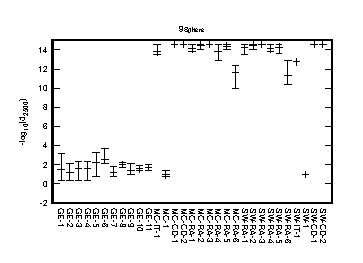
\includegraphics[width=\textwidth]{Sphere-e.eps}
\end{frame}

\begin{frame}
	\frametitle{Función de Ackley}
	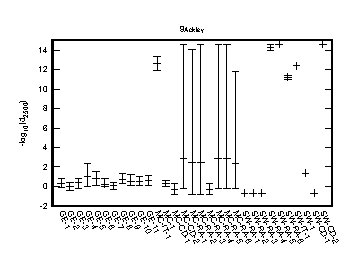
\includegraphics[width=\textwidth]{Ackley-e.eps}
\end{frame}

\begin{frame}
	\frametitle{Función de Booth}
	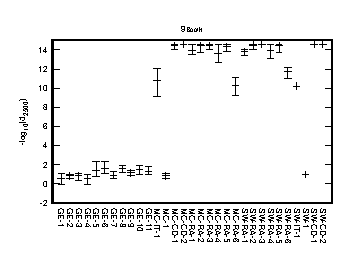
\includegraphics[width=\textwidth]{Booth-e.eps}
\end{frame}

\begin{frame}
	\frametitle{Función de Rosenbrock}
	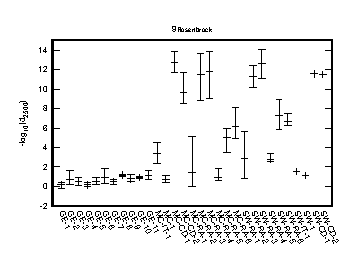
\includegraphics[width=\textwidth]{Rosenbrock-e.eps}
\end{frame}

\begin{frame}
	\frametitle{Función de Easom}
	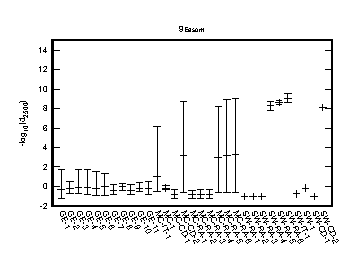
\includegraphics[width=\textwidth]{Easom-e.eps}
\end{frame}

\begin{frame}
	\frametitle{Función de Beale}
	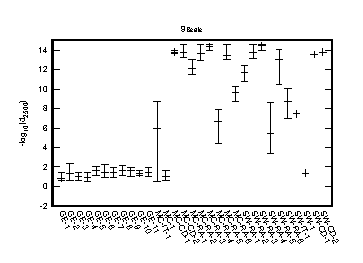
\includegraphics[width=\textwidth]{Beale-e.eps}
\end{frame}

\section{MPCOTool}

\begin{frame}
	\frametitle{Multi-Purposes Calibration and Optimization Tool}
	\begin{itemize}
		\item Código en lenguaje C
		\item Repositorio \url{https://github.com/jburguete/mpcotool}
		\item Utilidades requeridas para compilar el ejecutable
			\begin{itemize}
				\item Compilador de C: GCC o CLang
				\item Utilidades de configuración: Automake, Autoconf y
					PKGConfig
				\item Utilidad de control: GNUMake
			\end{itemize}
	\end{itemize}
\end{frame}

\begin{frame}
	\frametitle{Multi-Purposes Calibration and Optimization Tool}
	\begin{itemize}
		\item Código en lenguaje C
		\item Repositorio \url{https://github.com/jburguete/mpcotool}
		\item Utilidades requeridas para compilar el ejecutable
		\item Librerías externas libres
		\begin{itemize}
			\item Libxml2: fichero principal de entrada en formato XML
			\item GSL: generar números aleatorios
			\item GLib: análisis de plantillas de ficheros de entrada y para paralelizar en los diferentes procesadores de la máquina
			\item JSON-GLib: fichero principal de entrada en formato JSON
			\item GTK+3: interfaz gráfica interactiva
			\item OpenMPI o MPICH: paralelización en múltiples computadoras
		\end{itemize}
	\end{itemize}
\end{frame}

\begin{frame}
	\frametitle{Multi-Purposes Calibration and Optimization Tool}
	\begin{itemize}
		\item Código en lenguaje C
		\item Repositorio \url{https://github.com/jburguete/mpcotool}
		\item Utilidades requeridas para compilar el ejecutable
		\item Librerías externas
		\item Versiones en inglés, español, francés y alemán
		\item Multiplataforma
		\begin{itemize}
			\item Linux (Debian, Ubuntu, Fedora, OpenSUSE)
			\item Microsoft Windows 7 y 8.1
			\item BSD (FreeBSD, OpenBSD, NetBSD, DragonflyBSD, Debian kFreeBSD)
			\item Hurd (Debian)
		\end{itemize}
	\end{itemize}
\end{frame}

\begin{frame}
	\frametitle{Modo de uso}
	\begin{itemize}
		\item Modo de comandos
	\end{itemize}
.$/$mpcotoolbin [-nthreads X] [-seed S] fichero\_de\_entrada.xml
[fichero\_de\_resultados] [fichero\_de\_variables]
\end{frame}

\begin{frame}
	\frametitle{Modo de uso}
	\begin{itemize}
		\item Modo de comandos
		\item Paralelización en varias computadoras con MPI
	\end{itemize}
mpirun [MPI options] .$/$mpcotoolbin [-nthreads X] [-seed S] fichero\_de\_entrada.xml
[fichero\_de\_resultados] [fichero\_de\_variables]
\end{frame}

\begin{frame}
	\frametitle{Modo de uso}
	\begin{itemize}
		\item Modo de comandos
		\item Paralelización en varias computadoras con MPI
		\item Sintaxis del programa de simulación
	\end{itemize}
.$/$simulador fichero\_de\_entrada\_1 [fichero\_de\_entrada\_2] [...]
fichero\_de\_salida
\end{frame}

\begin{frame}
	\frametitle{Modo de uso}
	\begin{itemize}
		\item Modo de comandos
		\item Paralelización en varias computadoras con MPI
		\item Sintaxis del programa de simulación
		\item Sintaxis del programa de evaluación
	\end{itemize}
.$/$evaluador fichero\_simulado fichero\_experimental fichero\_de\_resultados
\end{frame}

\begin{frame}
	\frametitle{Aplicación con interfaz gráfica de usuario interactiva}
	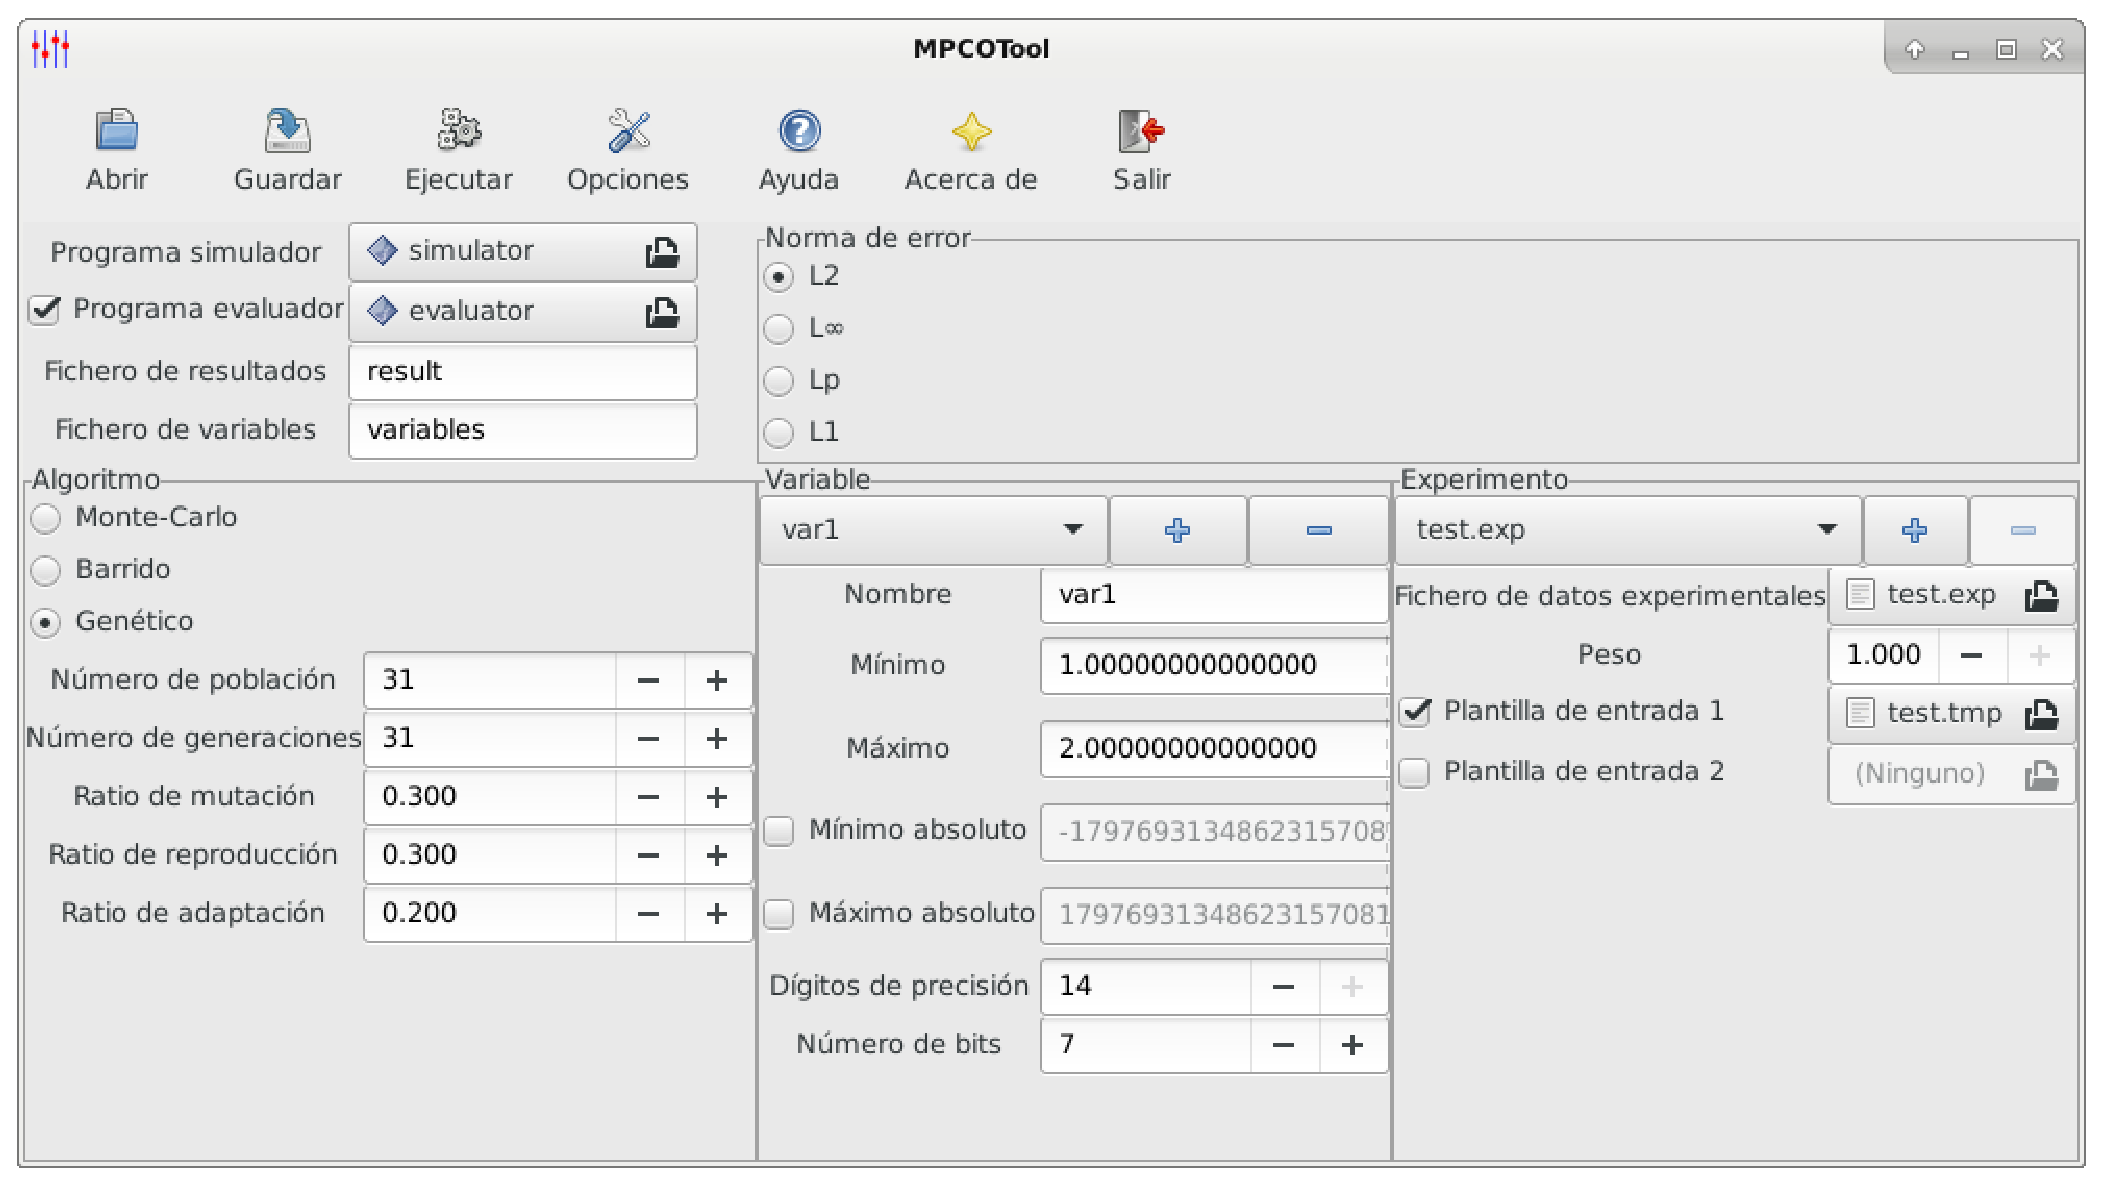
\includegraphics[width=\textwidth]{mpcotool-es.eps}
\end{frame}

\begin{frame}
	\frametitle{Fichero principal de entrada}
\psset{xunit=0.4mm,yunit=0.4mm}
\PSPICTURE{0}{-115}{280}{25}
{
	\tiny
	\psframe(0,-5)(280,25)
	\psline(40,-5)(40,25)
	\rput(20,20){\bf optimize}
	\rput(60,20){\bf simulator}
	\rput(95,20){\bf algorithm}
	\rput(130,20){evaluator}
	\rput(165,20){nsimulations}
	\rput(205,20){niterations}
	\rput(240,20){tolerance}
	\rput(265,20){nbest}
	\rput(60,10){threshold}
	\rput(95,10){npopulation}
	\rput(135,10){ngenerations}
	\rput(170,10){mutation}
	\rput(205,10){reproduction}
	\rput(240,10){adaptation}
	\rput(265,10){seed}
	\rput(60,0){direction}
	\rput(95,0){nsteps}
	\rput(130,0){nestimates}
	\rput(170,0){relaxation}
	\rput(200,0){norm}
	\rput(217,0){p}
	\rput(235,0){result}
	\rput(260,0){variables}
	\psline(20,-5)(20,-15)(40,-15)
	\psframe(40,-20)(280,-10)
	\psline(80,-20)(80,-10)
	\rput(60,-15){\bf experiment}
	\rput(95,-15){\bf name}
	\rput(125, -15){\bf template$_\mathbf{1}$}
	\rput(160,-15){template$_2$}
	\rput(195,-15){$\cdots$}
	\rput(230,-15){template$_n$}
	\rput(260,-15){weight}
	\psline(20,-15)(20,-25)
	\rput(140,-30){$\cdots$}
	\psline(20,-35)(20,-45)(40,-45)
	\psframe(40,-50)(280,-40)
	\psline(80,-50)(80,-40)
	\rput(60,-45){\bf experiment}
	\rput(95,-45){\bf name}
	\rput(125,-45){\bf template$_\mathbf{1}$}
	\rput(160,-45){template$_2$}
	\rput(195,-45){$\cdots$}
	\rput(230,-45){template$_n$}
	\rput(260,-45){weight}
	\psline(20,-45)(20,-65)(40,-65)
	\psframe(40,-75)(280,-55)
	\psline(80,-75)(80,-55)
	\rput(60,-60){\bf variable}
	\rput(95,-60){\bf name}
	\rput(120,-60){\bf minimum}
	\rput(152.5,-60){\bf maximum}
	\rput(195,-60){absolute\_minimum}
	\rput(250,-60){absolute\_maximum}
	\rput(100,-70){precision}
	\rput(130,-70){nsweeps}
	\rput(155,-70){nbits}
	\rput(175,-70){step}
	\psline(20,-65)(20,-80)
	\rput(140,-85){$\cdots$}
	\psline(20,-90)(20,-105)(40,-105)
	\psframe(40,-115)(280,-95)
	\psline(80,-115)(80,-95)
	\rput(60,-100){\bf variable}
	\rput(95,-100){\bf name}
	\rput(120,-100){\bf minimum}
	\rput(152.5,-100){\bf maximum}
	\rput(195,-100){absolute\_minimum}
	\rput(250,-100){absolute\_maximum}
	\rput(100,-110){precision}
	\rput(130,-110){nsweeps}
	\rput(155,-110){nbits}
	\rput(175,-110){step}
}
\end{frame}

\begin{frame}
	\frametitle{Ficheros de plantilla}
	\begin{itemize}
		\item Se requieren $N_{experimentos}\times N_{entradas}$ ficheros de
			plantilla
		\item MPCOTool analiza estas plantillas para generar ficheros de entrada
			de cada simulación:
		\begin{itemize}
			\item[@variableX@]: se reemplaza por la etiqueta asociada al $X$-ésima parámetro
	empírico definido en el fichero principal de entrada.
\item[@valueX@]: se reemplaza por el valor asociado al $X$-ésima parámetro
	empírico calculado por el algoritmo de optimización usando los datos
	definidos en el fichero principal de entrada.
		\end{itemize}
	\end{itemize}
\end{frame}

\begin{frame}
	\frametitle{Modo de operación}
\psset{xunit=0.4mm,yunit=0.4mm}
\PSPICTURE{-20}{-115}{260}{55}
{
	\tiny
	\rput(10,50){Entrada principal}
	\psframe(-20,45)(40,55)
	\psline{->}(40,50)(50,50)
	\rput(10,25){Plantilla primera}
	\psframe(-20,20)(40,30)
	\psline{->}(40,25)(50,25)
	\psline[linestyle=dotted,dotsep=1pt]{->}(50,25)(90,25)
	\rput(10,15){$\cdots$}
	\rput(10,5){Plantilla $n$-ésima}
	\psframe(-20,0)(40,10)
	\psline{->}(40,5)(50,5)
	\psline[linestyle=dotted,dotsep=1pt]{->}(50,5)(90,5)
	\rput(10,-35){$\cdots$}
	\rput(10,-75){Plantilla $(N\,n)$-ésima}
	\psframe(-20,-70)(40,-80)
	\psline{->}(40,-75)(50,-75)
	\psline[linestyle=dotted,dotsep=1pt]{->}(50,-75)(90,-75)
	\rput(70,50){MPCOTool}
	\psframe(50,-95)(90,55)
	\rput(70,-110){Función objetivo}
	\psframe(35,-105)(105,-115)
	\psline{->}(70,-95)(70,-105)
	\psline{->}(90,25)(100,25)
	\psline{->}(90,5)(100,5)
	\psline{->}(90,-55)(100,-55)
	\psline{->}(90,-75)(100,-75)
	\rput(125,5){Entrada $n$-ésima}
	\psframe(100,0)(150,10)
	\psline{->}(150,5)(160,5)
	\rput(125,15){$\cdots$}
	\rput(125,25){Entrada primera}
	\psframe(100,20)(150,30)
	\psline{->}(150,25)(155,25)(155,5)
	\rput(180,5){Simulador}
	\psframe(160,0)(200,10)
	\psline[linestyle=dashed,dash=2pt 1pt]{->}(175,10)(175,20)
	\psline[linestyle=dashed,dash=2pt 1pt]{->}(200,5)(210,7.5)
	\rput(180,25){Resultados}
	\psframe[linestyle=dashed,dash=3pt 1pt](160,20)(200,30)
	\psline[linestyle=dashed,dash=2pt 1pt]{->}(200,25)(210,30)
	\rput(180,45){Datos del}
	\rput(180,40){experimento}
	\psframe(160,35)(200,50)
	\psline[linestyle=dashed,dash=2pt 1pt]{->}(200,42.5)(210,30)
	\psline[linestyle=dashed,dash=2pt 1pt]{->}(160,42.5)(155,42.5)(155,25)
	\rput(230,30){Evaluador}
	\psline[linestyle=dashed,dash=2pt 1pt]{->}(230,25)(230,15)
	\psframe[linestyle=dashed,dash=3pt 1pt](210,25)(250,35)
	\rput(230,10){Valor}
	\rput(230,5){objetivo}
	\psframe(210,0)(250,15)
	\psline{->}(250,7.5)(260,7.5)(260,-90)(90,-90)
	\psline[linestyle=dotted,dotsep=1pt]{->}(90,-90)(70,-90)(70,-95)
	\rput(125,50){Experimento primero}
	\psframe[linestyle=dotted](95,-5)(255,55)
	\rput(175,-15){$\cdots$}
	\rput(125,-75){Entrada $n$-ésima}
	\psframe(100,-80)(150,-70)
	\psline{->}(150,-75)(160,-75)
	\rput(125,-65){$\cdots$}
	\rput(125,-55){Entrada primera}
	\psframe(100,-60)(150,-50)
	\psline{->}(150,-55)(155,-55)(155,-75)
	\rput(180,-75){Simulador}
	\psframe(160,-80)(200,-70)
	\psline[linestyle=dashed,dash=2pt 1pt]{->}(180,-70)(180,-60)
	\psline[linestyle=dashed,dash=2pt 1pt]{->}(200,-75)(210,-72.5)
	\rput(180,-55){Resultados}
	\psframe[linestyle=dashed,dash=3pt 1pt](160,-60)(200,-50)
	\psline[linestyle=dashed,dash=2pt 1pt]{->}(200,-55)(210,-50)
	\rput(180,-35){Datos del}
	\rput(180,-40){experimento}
	\psframe(160,-30)(200,-45)
	\psline[linestyle=dashed,dash=2pt 1pt]{->}(200,-37.5)(210,-50)
	\psline[linestyle=dashed,dash=2pt 1pt]{->}(160,-37.5)(155,-37.5)(155,-55)
	\rput(230,-50){Evaluador}
	\psline[linestyle=dashed,dash=2pt 1pt]{->}(230,-55)(230,-65)
	\psframe[linestyle=dashed,dash=3pt 1pt](210,-55)(250,-45)
	\rput(230,-70){Valor}
	\rput(230,-75){objetivo}
	\psframe(210,-80)(250,-65)
	\psline(250,-72.5)(260,-72.5)
	\rput(125,-30){Experimento $N$-ésimo}
	\psframe[linestyle=dotted](95,-85)(255,-25)
}
\end{frame}

\begin{frame}
	\frametitle{Normas de error}
	\[L_2:\quad J=\sqrt{\sum_{i=1}^{N_{exp}}\ABS{w_i\,o_i}^2},\]
	\[L_\infty:\quad J=\max_{i=1}^{N_{exp}}\ABS{w_i\,o_i},\]
	\[L_p:\quad J=\sqrt[p]{\sum_{i=1}^{N_{exp}}\ABS{w_i\,o_i}^p},\]
	\[L_1:\quad J=\sum_{i=1}^{N_{exp}}\ABS{w_i\,o_i},\]
\end{frame}

\section{Aplicaciones prácticas}

\begin{frame}
	\begin{itemize}
		\item Optimización de los horarios de apertura de compuertas en el tramo
			nuevo del Canal de la Violada
		\item Calibración de los coeficientes de rozamiento e infiltración en
			riego por surcos
		\item Calibración de los coeficientes de distribución de tamaño de gota
			y de rozamiento en riego por aspersión
		\item Calibración de los coeficientes de funcionamiento del movimiento
			de torres de pivots
	\end{itemize}
\end{frame}

\section{Conclusiones}

\begin{frame}
\begin{itemize}
	\item MPCOTool es una utilidad para calibración/optimización fácil,
		flexible, intuitiva, ...
	\item Implementa muchos de los algoritmos más útiles de optimización
	\item Es capaz de utilizar paralelizadamente de una forma sencilla para el
		usuario todos los recursos computacionales disponibles
\end{itemize}
\end{frame}

\end{document}

\begin{frame}
	\begin{itemize}
		\item DEC VAX
		\item Zilog Z80 (Spectrum, Commodore)
		\item Motorola 68000
		\item Intel 8086
	\end{itemize}
\end{frame}

\begin{frame}
	\begin{center}
		\psset{xunit=1pt}
		\psset{yunit=1pt}
		\begin{pspicture}(200pt,150pt)
			\tiny
			\psframe(0,0)(200,150)
			\rput(100,145){Intel Core 64 bits}
			\psframe(5,5)(100,140)
			\rput(52.5,135){Pentium 32 bits}
			\psframe(10,10)(95,130)
			\rput(52.5,125){80486 32 bits}
			\psframe(60,15)(90,120)
			\rput(75,75){80387}
			\rput(75,60){32 bits}
			\psframe(15,15)(55,120)
			\rput(35,115){80386 32 bits}
			\psframe(20,20)(50,75)
			\rput(35,65){80286}
			\rput(35,60){16 bits}
			\psframe(25,25)(45,50)
			\rput(35,40){8086}
			\rput(35,35){16 bits}
			\psframe(105,5)(195,140)
			\rput(150,72.5){AMD64 (x86\_64)}
		\end{pspicture}
	\end{center}
\end{frame}

\subsection{Procesadores RISC}
\begin{frame}
	\begin{itemize}
		\item RISC: Reduced Instruction Set Computer
	\end{itemize}
	\begin{center}
		\psset{xunit=1.5pt}
		\psset{yunit=1.5pt}
		\begin{pspicture}(45pt,0pt)(375pt,150pt)
			\tiny
			\rput(80,95){Procesador CISC}
			\psframe(30,0)(130,100)
			\rput(55,70){Decodificador}
			\psframe(40,50)(70,90)
			\rput(55,25){Caché}
			\psframe(40,10)(70,40)
			\rput(100,70){ALU}
			\psframe(80,50)(120,90)
			\rput(100,5){Registros}
			\multido{\i=10+5,\ii=15+5}{6}{\psframe(80,\i)(120,\ii)}
			\multido{\r=52.5+5}{8}{\psline(70,\r)(80,\r)}
			\multido{\r=41.875+3.75}{8}{\psline(\r,40)(\r,50)}
			\multido{\r=82.5+5}{8}{\psline(\r,40)(\r,50)}
			\rput(189,79){Procesador RISC}
			\psframe(150,0)(228,84)
			\rput(172,62){Caché}
			\psframe(160,50)(184,74)
			\rput(206,62){ALU}
			\psframe(194,50)(218,74)
			\rput(198,5){Registros}
			\multido{\i=10+5,\ii=15+5}{6}{\psframe(178,\i)(218,\ii)}
			\multido{\r=51.5+3}{8}{\psline(184,\r)(194,\r)}
			\multido{\r=180.5+5,\rr=195.5+3}{8}{\psline(\r,40)(\rr,50)}
		\end{pspicture}
	\end{center}
\end{frame}

\begin{frame}
	\begin{itemize}
		\item Alpha $\rightarrow$ ShenWei
		\item SPARC
		\item Power $\rightarrow$ PowerPC
		\item ARM
		\item MIPS (dispositivos electrónicos: consolas, módems/routers,
			tarjetas de red, controladores de disco, programadores,
			data loggers, cámaras de foto o vídeo, decodificadores,
			electrodomésticos, coches, aviones, naves espaciales, ...)
	\end{itemize}
\end{frame}

\begin{frame}
	\begin{itemize}
		\item Híbrido CISC/RISC
	\end{itemize}
	\begin{center}
		\begin{pspicture}(135pt,60pt)
			\psset{xunit=1.5pt}
			\psset{yunit=1.5pt}
			\tiny
			\psframe(0,0)(40,40)
			\rput(20,20){Decodificador}
			\psframe(50,0)(90,40)
			\rput(70,20){RISC}
			\multido{\r=2.5+5}{8}{\qline(40,\r)(50,\r)}
		\end{pspicture}
	\end{center}
	\TABLE{c|cc}
	{
		& CISC & RISC \\
		\hline
		Velocidad & Similar & Similar \\
		Consumo energético & Mayor & Menor \\
		Calentamiento & Mayor & Menor \\
		Precio & Mayor & Menor \\
		Tamaño ejectubles & Menor & Mayor \\
		Uso RAM & Menor & Mayor
	}
\end{frame}

\section{Procesadores ARM}
\subsection{Historia}
\begin{frame}
	\begin{itemize}
		\item Acorn creó el primer procesador ARM (Acorn RISC Machine) de 32
			bits en 1985
		\item En 1990 se venden participaciones de la división de diseño de los
			ARM a las empresas Apple y VLSI $\Rightarrow$ Advanced RISC Machine
			y se forma ARM Holding
		\item A día de hoy se han vendido $\approx$ 60 mil millones de unidades
	\end{itemize}
\end{frame}

\subsection{Fabricación}
\begin{frame}
	\begin{itemize}
		\item ARM Holding sólo diseña procesadores ARM. Vende licencias de
			fabricación pero no los fabrica.
		\item Fabricantes: Samsung, Apple, NVIDIA, Broadcom, Texas Instruments,
			...
		\item Intel y AMD poseen licencias desde hace muchos años pero no han
			entrado todavía en la fabricación
	\end{itemize}
\end{frame}

\subsection{Usos}
\begin{frame}
	\begin{itemize}
		\item dispositivos electrónicos: consolas, módems/routers,
			tarjetas de red, controladores de disco, programadores,
			data loggers, cámaras de foto o vídeo, decodificadores,
			electrodomésticos, coches, aviones, naves espaciales, ...
		\item servidores
		\item miniordenadores
		\item $\approx70\%$ de tablets (android)
		\item $>99\%$ de teléfonos móviles
	\end{itemize}
\end{frame}

\subsection{Sistemas operativos}
\begin{frame}
	\begin{itemize}
		\item Linux $\Rightarrow$ Android
		\item BSD (FreeBSD, OpenBSD, NetBSD) $\Rightarrow$ Mac OS
		\item Windows CE, Mobile, Phone $\Rightarrow$ 10
	\end{itemize}
\end{frame}

\section{Miniordenadores}
\subsection{Productos}
\begin{frame}
	\begin{itemize}
		\item Raspberry
		\item Rikomagic
		\item Odroid
		\item MeegoPad
	\end{itemize}
\end{frame}

\subsection{Prestaciones}
\begin{frame}
\begin{center}
	\tiny
	\begin{tabular}{c|ccccccc}
		& Precio & Procesador & Núcleos & Velocidad & RAM & Tarjeta &
		Potencia\\
		\hline
		Raspberry Pi 2 & +40\euro & ARM & 4 & 0.9GHz & 1GB & MicroSD 8-64GB &
			10W \\
		Rikomagic MK802V & 125\euro & ARM & 4 & 1.8GHz & 2GB & Flash 16GB &
			10W \\
		Odroid C1 & +60\euro & ARM & 4 & 1.5GHz & 1GB & 8-64GB & 10W \\
		Odroid XU3 Lite & +180\euro & ARM & 8 & 1.8-1.3GHz & 2GB & 8-64GB &
			20W\\
		MeegoPad & 130\euro & Atom & 4 & 1.8GHz & 2GB & MicroSD 16-32G & 10W \\
		Portátil Thinkpad & 600\euro & i7 & 2 & 2.6GHz & 4GB & Disco 200GB &
			85W
	\end{tabular}
\end{center}
\end{frame}

\begin{frame}
\begin{center}
	\tiny
	\begin{tabular}{c|ccccc}
		& Precio & Potencia & Fractal & Surcos & Sistema \\
		\hline
		Rikomagic MK802V & 125\euro & 10W & 204 s & 38 s &
			ARM Xubuntu Linux 15 (32 bits) \\
		Odroid XU3 Lite & +180\euro & 20W & 135 s & 58 - 129 s &
			ARM Xubuntu Linux 14 (32 bits) \\
		Portátil Thinkpad & 600\euro & 85W & 60 s & 10 s &
			AMD64 Debian Linux 8 (64 bits)
	\end{tabular}
\end{center}
\end{frame}

\subsection{Software}
\begin{frame}
\begin{itemize}
	\item Pros
	\begin{itemize}
		\item Android: mejores drivers
		\item Linux: funcionan prácticamente todos los programas
	\end{itemize}
	\item Contras
	\begin{itemize}
		\item Linux: instalaciones bastante experimentales
		\item Arranque grabado en una partición de la tarjeta
		\item Dificultad de actualización
	\end{itemize}
\end{itemize}
\end{frame}

\section{Conclusiones}
\begin{frame}
\begin{itemize}
	\item Estamos viviendo una revolución tecnológica con los teléfonos móviles
		y las tablets
	\item En buena medida es responsable el procesador ARM, un diseño de
		mediados de los 80
	\item Los procesadores ARM son procesadores RISC, más simples, más
		eficientes energéticamente y más baratos de fabricar
	\item Una aplicación que puede ser interesante en el futuro próximo es la de
		los miniordenadores ARM. Son muy compactos, muy baratos y consumen muy
		poca energía. Podrían competir como portátiles, data loggers,
		programadores, ...
\end{itemize}
\end{frame}

\begin{frame}
	\begin{center}
		\LARGE ¡GRACIAS!\\
		\includegraphics[width=6cm]{Huerto.eps}
		\includegraphics[width=6cm]{Vehiculo.eps}
	\end{center}
\end{frame}

\end{document}
